\documentclass[11pt]{article}

\usepackage[a4paper,margin=1in]{geometry}
\usepackage{amsmath,amssymb}
\usepackage{hyperref}
\hypersetup{
    colorlinks,
    citecolor=blue,
    filecolor=black,
    linkcolor=blue,
    urlcolor=blue
}
\usepackage{graphicx}
\usepackage{tikz}
\usetikzlibrary{arrows.meta}



\title{\textbf{Quantitative Reasoning and Mathematical Thinking (QRMT): End-of-sem project ideas}}
\date{}
\begin{document}
\maketitle

You may consider one or more of the following project suggestions for your end-sem QRMT project. You can of course discuss your own project ideas with the teaching team. The grading will depend on both the quality of your solution and the difficulty level of the project, as perceived by the teaching team.

\section{Estimating quantities}

Estimate how much plastic and paper are consumed in Ashoka weekly? Describe your method and comment on how accurate is your estimate?

\section{Estimating heights in the wild}
\begin{center}
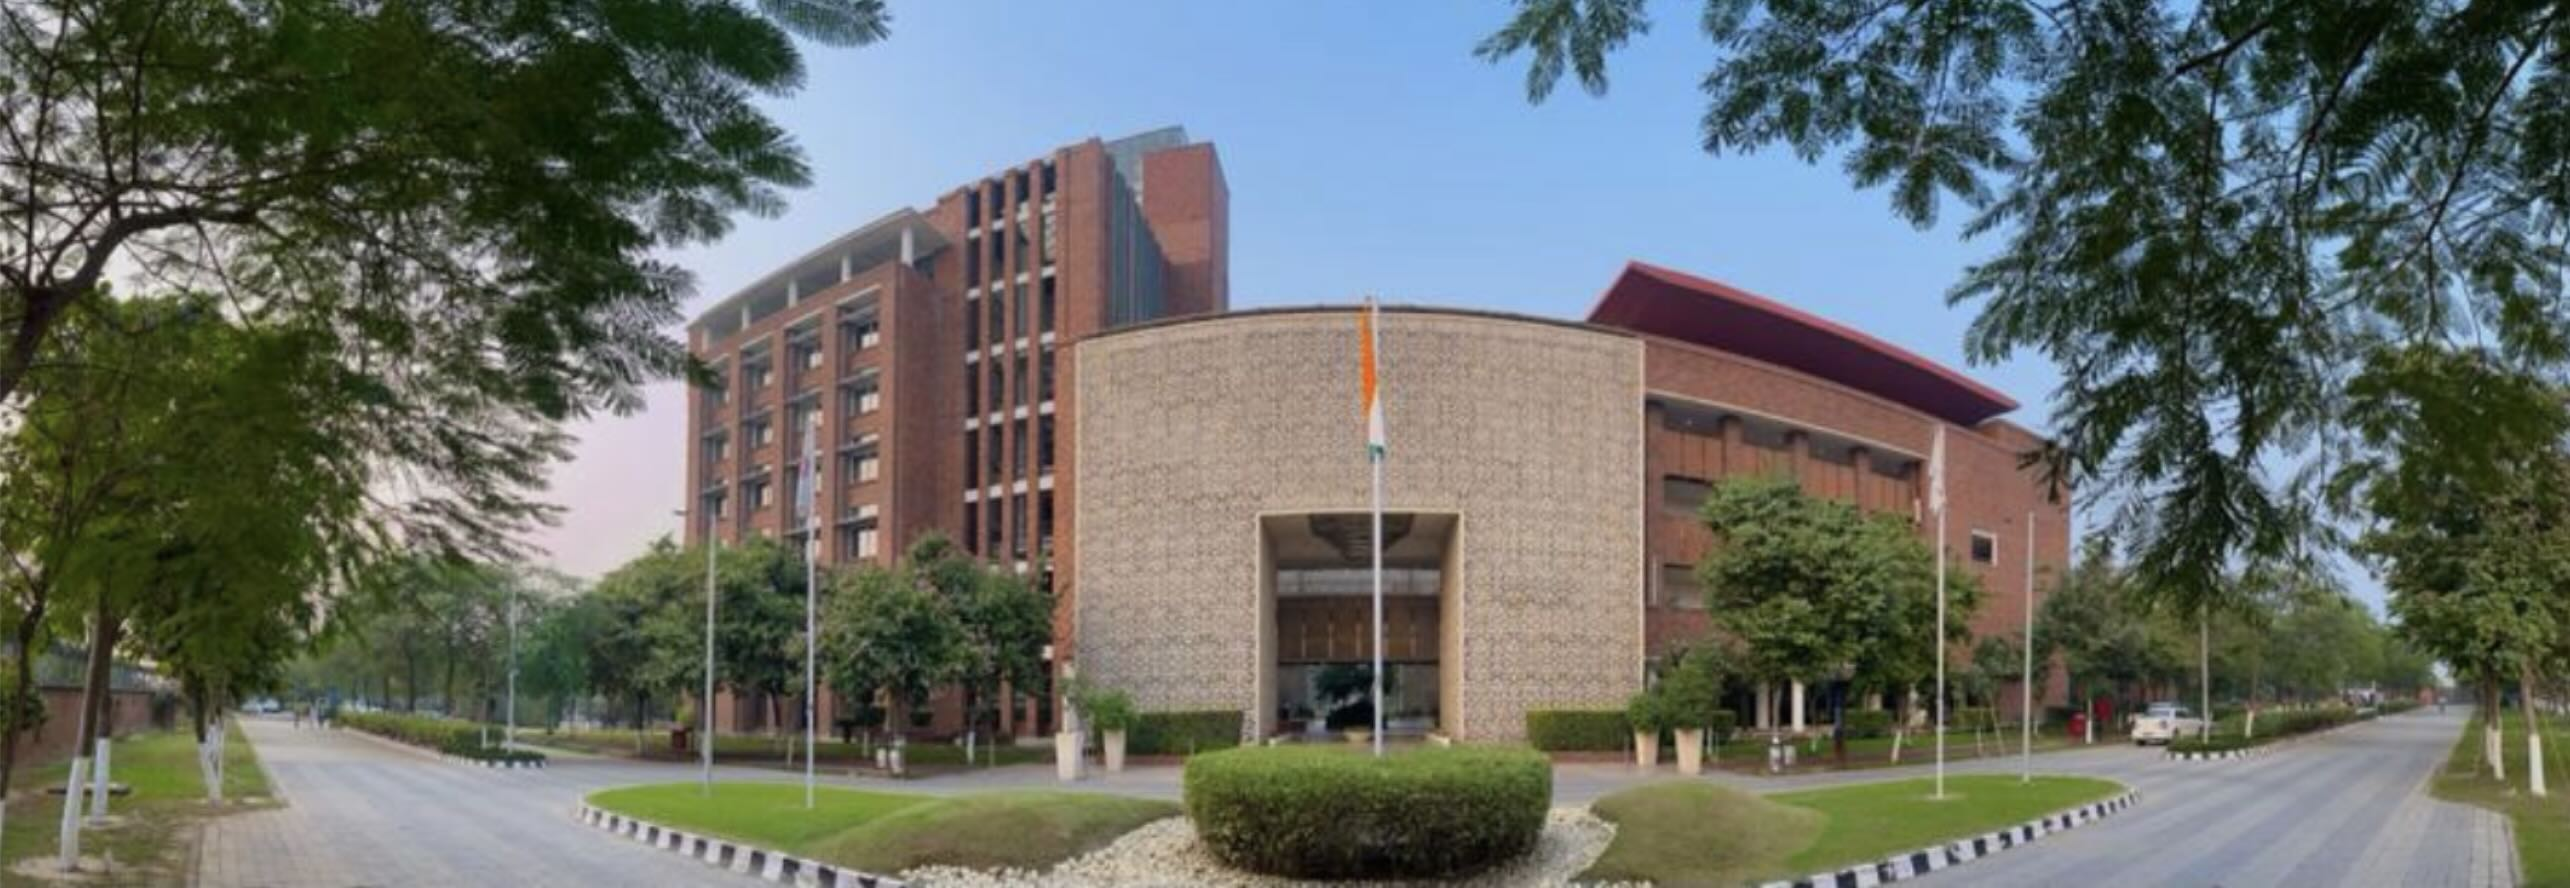
\includegraphics[width=3.0in]{images/flagpost.jpg}
\end{center}

Measure the height of the flag post outside the admin block in the units of your own height. Alternatively, you can can find the height of  your favourite lamp post in Ashoka. Describe your method clearly stating all  assumptions.  What would be the various sources of errors in your measurement method. Suppose you make a $0.5\%$ error in measuring your own height, what will be the error in the height of the flag post? Climbing posts, climbing on ladders, climbing on people's shoulders etc. are not allowed. Instead, you may watch \href{https://youtu.be/bkNMM8uiMww?si=vBXfZsTu-Frzyv6G}{this video} for inspiration.

\section{Estimating areas and numbers}

Estimate the number of rectangular red bricks in the front face of the AC04. Describe your method clearly stating all the assumptions? How accurate is your estimate? Climbing the front face of AC04  or rappelling are not allowed. The video above may help.

\section{Estimating the area of the AC04 trellis}
\begin{center}
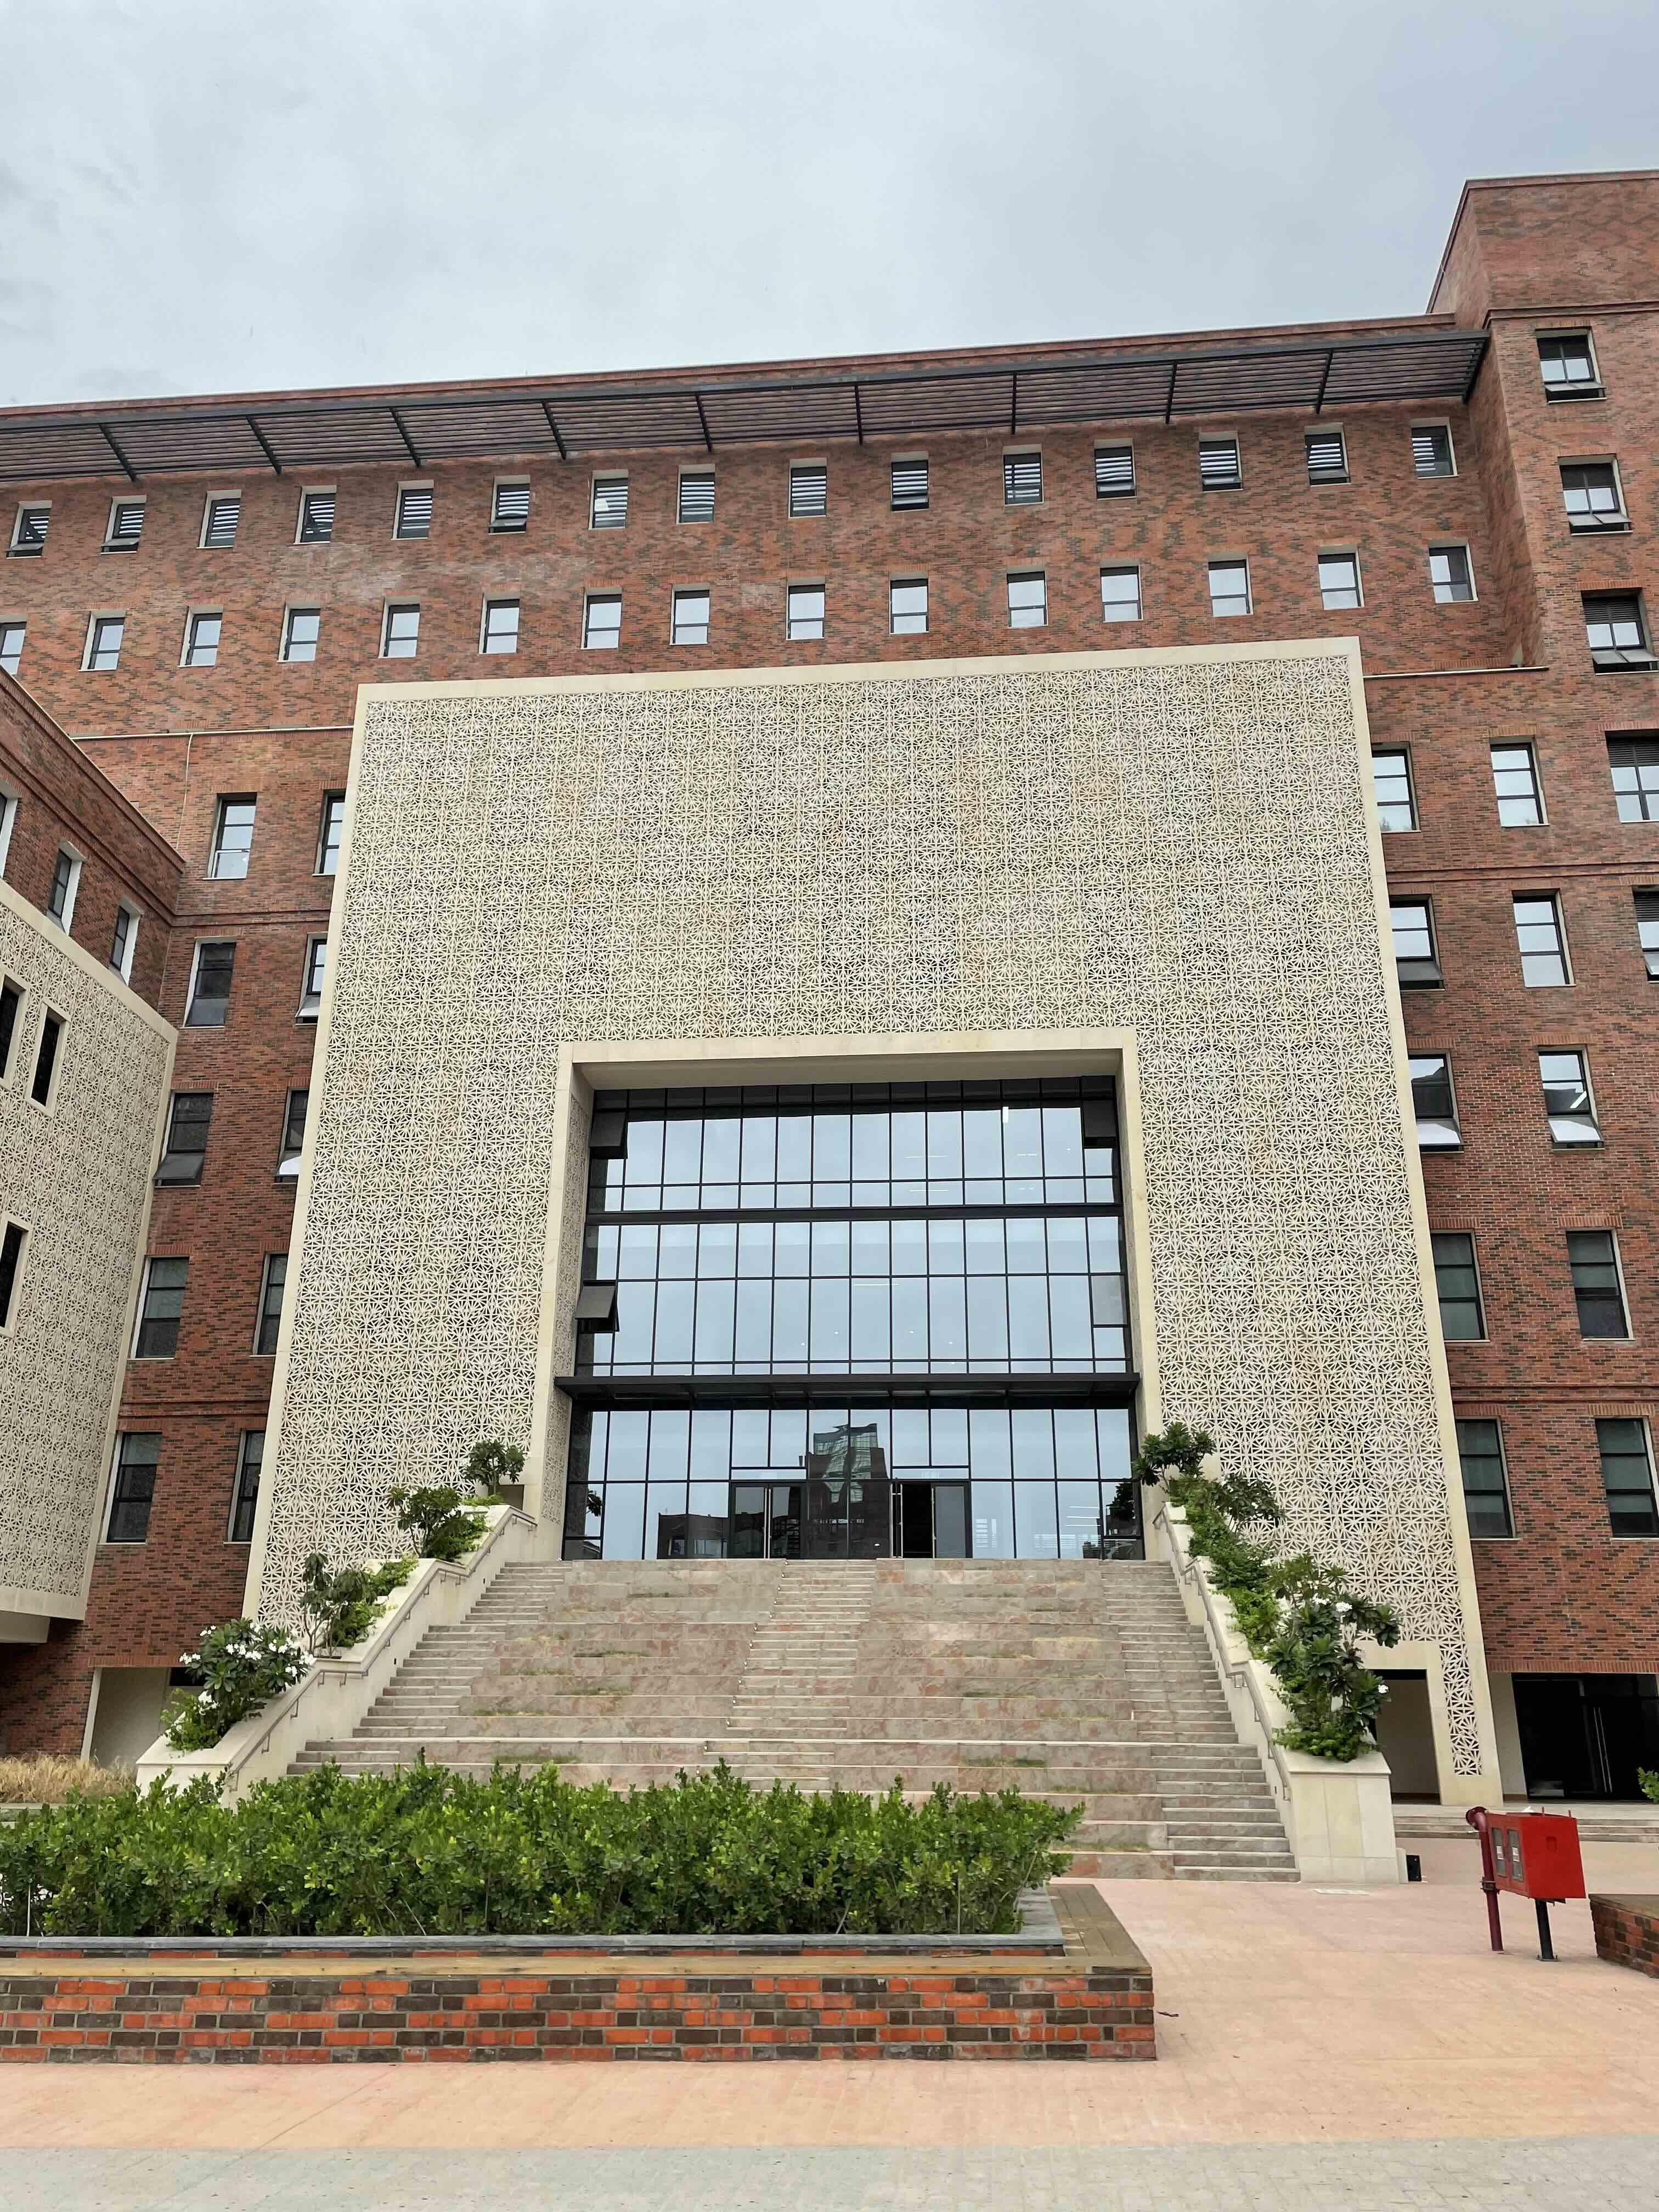
\includegraphics[width=2.0in]{images/AC04.jpg}
\end{center}


Estimate the area of the big trellis structure in the front face of AC04, counting only the material and not the gaps in between. Please describe your method clearly stating all assumptions. How accurate is your estimate? Climbing the front face of AC04 is not allowed. The video above may help.

\section{$ut +\frac{1}{2}gt^2$}
\begin{center}
\includegraphics[width=1.5in]{images/galileo.jpeg}
\end{center}

It is said that the celebrated scientist \href{https://en.wikipedia.org/wiki/Galileo_Galilei}{Galileo Galilei} invented the famous \emph{time} vs \emph{displacement} equation $ut + \frac{1}{2}at^2$. The formula gives the displacement when $u$ is the initial velocity (zero for free fall from rest), $a$ is the acceleration (approximately 9.81 $m/sec^2$ for free fall), and $t$ is the elapsed time. In the true spirit of \emph{data science}, create a \emph{time} vs \emph{displacement} measurement table from which we may verify or even re-discover the formula. How many rows in the table will you require? How accurately do you need to measure? Does your measurement method achieve the required accuracy? How would Galileo have measured, if at all (the folk lore is that he dropped objects from the Leaning Tower of Pisa to discover the law)? Visiting Pisa, climbing atop buildings etc. are not allowed.

\section{Determining the latitude of Ashoka University}


The height of the Sun at \emph{local solar noon} depends only on the
\textbf{latitude} of the observer and the \textbf{declination} of the Sun on that
date. By measuring the shortest shadow of a vertical stick\footnote{This project may be untenable because of pollution.}, one can estimate
the solar altitude and hence deduce the latitude. This method is essentially
what \href{https://youtu.be/Mw30CgaXiQw?si=pzCINbV5dehU2Vf2}{Eratosthenes used over 2200 years ago}\footnote{You may also try calculating the circumference of the earth by Eratosthenes' method.}. You can try to measure the latitude of Ashoka university using the following sketch of a method. Please fill in the details and explain the reason for inaccuracies in your measurements, if any.

\subsection*{Experimental Setup}

Place a vertical stick (a \emph{gnomon}) of known height $H$ on level ground.
To ensure verticality, use a plumb line or a spirit level. Observe the shadow
around midday and mark the tip every few minutes. The shadow will
decrease in length until solar noon, then increase. Record the \emph{shortest}
shadow length $L$.


\begin{figure}[h]
  \centering
  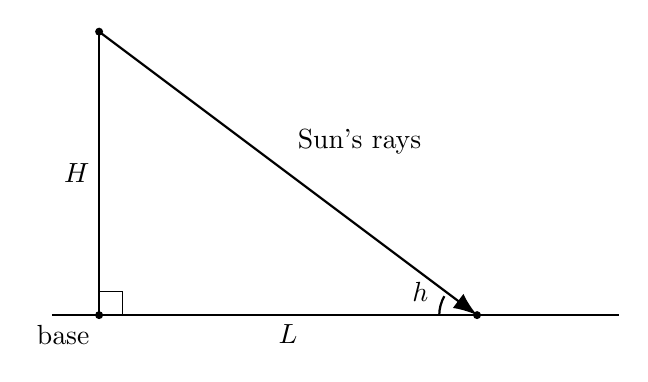
\begin{tikzpicture}[scale=1.2]

    % Ground line
    \draw[thick] (-0.5,0) -- (5.5,0);
    %\node[below] at (2.5,0) {ground};

    % Stick (gnomon)
    \draw[thick] (0,0) -- (0,3);
    \fill (0,0) circle (1.2pt);
    \fill (0,3) circle (1.2pt);
    \node[left] at (0,1.5) {$H$};
    \node[below left] at (0,0) {base};

    % Shadow (horizontal)
    \draw[thick] (0,0) -- (4,0);
    \fill (4,0) circle (1.2pt);
    \node[below] at (2,0) {$L$};
    %\node[below] at (4,0) {shadow tip};

    % Sun ray from top of stick
    \draw[thick,-{Latex[length=3mm]}] (0,3) -- (4,0);
    \node[above right] at (2,1.6) {Sun's rays};

    % Solar altitude angle h at shadow tip
    % Angle between horizontal (to left) and sun ray
    \draw (4,0) ++(-0.8,0) -- (4,0) -- ++(-0.6,0.45);
    % Angle arc
    \draw[thick]
      (4,0) ++(-0.4,0)
      arc[start angle=180,end angle=150,radius=0.4];
    \node at (3.4,0.25) {$h$};

    % Right-angle at base of stick
    \draw (0,0) ++(0.25,0) -- ++(0,0.25) -- ++(-0.25,0);

  \end{tikzpicture}
  \caption{Vertical stick of height $H$, shadow length $L$, and solar altitude angle $h$.}
\end{figure}

\subsection*{Solar Altitude from a Shadow}

At local solar noon, the Sun, the tip of the stick, and its shadow lie in a
vertical plane. The solar altitude angle $h$ (angle above the horizon) satisfies
\[
\tan h = \frac{H}{L}
\qquad\Rightarrow\qquad
h = \arctan\!\left(\frac{H}{L}\right).
\]

For example, if $H=1.0\,$m and $L=0.70\,$m, then
\[
h \approx \arctan(1/0.7) \approx 55^\circ.
\]

\subsection*{Solar Declination}

The solar declination $\delta$ is the Sun's ``latitude'' on the celestial
sphere. It depends only on the date:
\begin{itemize}
    \item March and September equinoxes: $\delta \approx 0^\circ$.
    \item June solstice: $\delta \approx +23.5^\circ$.
    \item December solstice: $\delta \approx -23.5^\circ$.
\end{itemize}
A table or website can give $\delta$ for any day of the year, but for many
classroom experiments these values suffice.

\subsection*{Relationship Between Latitude, Declination, and Altitude}

At local solar noon the relationship is
\[
h = 90^\circ - \lvert\,\varphi - \delta\,\rvert,
\]
where
\begin{itemize}
    \item $\varphi$ = observer's latitude (unknown),
    \item $\delta$ = solar declination (known from date),
    \item $h$ = solar altitude (measured from the shadow).
\end{itemize}

Rearranging gives
\[
\lvert\,\varphi - \delta\,\rvert = 90^\circ - h,
\]
and hence the two algebraic possibilities:
\[
\varphi = \delta \pm (90^\circ - h).
\]

The correct sign is chosen by noting whether, at solar noon, the Sun is
\emph{south} (typical in the northern hemisphere) or \emph{north}
(typical in the southern hemisphere).

\subsection*{Special Case: Measuring Near an Equinox}

For dates near the equinoxes, $\delta \approx 0^\circ$. The latitude in the
northern hemisphere is then
\[
\varphi \approx 90^\circ - h.
\]

\medskip
\noindent\textbf{Example.}
Suppose at the March equinox the minimum shadow of a 1\,m stick is
$L = 0.78\,$m.
Then
\[
h = \arctan\!\left(\frac{1}{0.78}\right) \approx 52^\circ,
\qquad
\varphi \approx 38^\circ \text{ N}.
\]

\subsection*{Role of Longitude}

Longitude does \emph{not} enter the geometric relation above. It affects only
the \emph{timing} of local solar noon. One can simply find solar noon
empirically as the moment of the \emph{shortest shadow}. Thus the experiment
requires no clocks and no prior knowledge of longitude.

\subsection*{Summary of the Procedure}

\begin{enumerate}
    \item Measure stick height $H$.
    \item Determine local solar noon by observing the shortest shadow.
    \item Measure minimum shadow length $L$.
    \item Compute $h = \arctan(H/L)$.
    \item Look up the solar declination $\delta$ for the date.
    \item Solve $\;h = 90^\circ - |\varphi - \delta|\;$ for $\varphi$.
\end{enumerate}

This simple method can locate your latitude to within one or two degrees with
careful measurement.

\section{Logical validity of arguments}
An argument is \emph{valid} (an \emph{entailment}) iff if we grant that the premises are all true, then the conclusion must also be true.
An invalid argument is a \emph{fallacy}.

Constructing a truth table is one way to check the validity.

What about?
\emph{``If Rahul drinks beer in Haryana, he is at least 25 years old. Rahul does not drink beer. Therefore, Rahul is not yet 25 years old''}?

\vspace{0.25in}
Here is a more complicated one  from Lewis Caroll:

\begin{enumerate}
\item \emph{All the dated letters in this room are written on blue paper.}
\item  \emph{None of them are in black ink, except those that are written in the third person. }
\item  \emph{I have not filed any of those that I can read.}
\item  \emph{None of those that are written on one sheet are undated.}
\item  \emph{All of those that are not crossed out are in black ink.}
\item  \emph{All of those that are written by Brown begin with “Dear Sir.”}
\item  \emph{All of those that are written on blue paper are filed.}
\item  \emph{None of those that are written on more than one sheet are crossed out.}
\item  \emph{None of those that begin with “Dear sir” are written in the third person. }
\end{enumerate}

\emph{Therefore, I cannot read any of Brown’s letters. }

\vspace{0.25in}
Can you (with some research) figure out a  general strategy for checking the validity of such arguments?

\section{Modelling rumour spread and experimental validation}

Rumours propagate through social contact much like infectious diseases.
This project invites you to (a) build a simple quantitative model of
rumour spread and (b) design an experiment in a controlled classroom
setting to validate the model. The aim is to explore how assumptions
about contact behaviour, probability, and network structure influence
the spread of information.

\subsection*{A Simple Discrete-Time Rumour Model}

Consider a population of $N$ students. At time $t$, each individual is
classified as:

\begin{itemize}
    \item \textbf{Ignorant} $I(t)$: has not heard the rumour.
    \item \textbf{Spreader} $S(t)$: currently forwarding the rumour.
    \item \textbf{Stifler} $R(t)$: knows the rumour but no longer spreads it.
\end{itemize}

Thus,
\[
I(t) + S(t) + R(t) = N.
\]

We assume discrete time steps $t=0,1,2,\dots$. Let each spreader contact
$c$ individuals per step (on average).

\subsection*{Contact assumptions}
\begin{itemize}
    \item Each contact with an ignorant person turns them into a
    spreader with probability $p$.
    \item Each contact with someone who already knows the rumour
    (spreader or stifler) causes the spreader to lose interest and
    become a stifler with probability $q$.
\end{itemize}

Using expected values, the approximate change in populations is

\[
\Delta S_+ \approx p c\, S(t)\,\frac{I(t)}{N}, \qquad
\Delta R_+ \approx q c\, S(t)\,\frac{S(t)+R(t)}{N}.
\]

Hence the discrete update equations are
\[
\begin{aligned}
I(t+1) &= I(t) - \Delta S_+, \\
S(t+1) &= S(t) + \Delta S_+ - \Delta R_+, \\
R(t+1) &= R(t) + \Delta R_+.
\end{aligned}
\]

With initial condition $I(0)=N-1$, $S(0)=1$, $R(0)=0$, one observes the
typical ``epidemic'' pattern: $S(t)$ rises to a peak and falls, while
$R(t)$ eventually saturates.

\subsection*{Network-Based Variant}

Instead of assuming that each person is equally likely to contact anyone
else, we may model the class as a \emph{network} (graph):

\begin{itemize}
    \item Nodes = students.
    \item Edges = communication pathways (friends, group chats, tutorial groups).
\end{itemize}

In each time step:
\begin{itemize}
    \item Each spreader contacts each neighbour with probability $p_c$.
    \item Ignorant neighbours become spreaders with probability $p$.
    \item Contacts with informed neighbours convert the spreader to a
    stifler with probability $q$.
\end{itemize}

This variant illustrates that network topology strongly influences the
speed and reach of rumour propagation (dense networks spread faster;
clustered networks may trap the rumour within communities).

\subsection*{Experimental Validation (Classroom Protocol)}

We outline an ethical, controlled experiment:

\subsubsection*{Step 1: Choose a benign rumour}
Use a clearly fictional statement, e.g.
\begin{quote}
``There may be a trial 7-minute break halfway through the next class.''
\end{quote}
Explain that this is part of a rumour-spread experiment and has no
official significance.

\subsubsection*{Step 2: Define a communication network}

Two options:
\begin{enumerate}
    \item \emph{Free communication:} Students use their normal channels
    (WhatsApp groups, face-to-face).
    \item \emph{Structured network:} Give each student a list of 4--5
    neighbours they may contact. This produces a controlled graph.
\end{enumerate}

\subsubsection*{Step 3: Launch the rumour}

Identify one or two source students. Provide them with the rumour and
ask them to share it only within the permitted network.

Each student keeps an anonymous log:
\begin{itemize}
    \item time they first heard the rumour,
    \item how many people told them,
    \item whether they forwarded it to others (and how many).
\end{itemize}

\subsubsection*{Step 4: Collect data}
After a fixed period (e.g.\ 48 hours), collect anonymised reports via a
web form.

You can estimate:
\[
K(t) = \text{number of students who knew the rumour by time } t,
\]
and possibly approximate $I(t), S(t), R(t)$ over time.

\subsection*{Step 5: Fit the model}

Use early-time growth to estimate an effective reproduction number
\[
R_{\text{eff}} \approx
\frac{\text{\# new knowers at time } t+1}
     {\text{\# knowers at time } t}
\]
and relate it to $c p$ in the model. Estimate when the rumour peaks and
compare the height and timing of this peak with your simulation.

\subsection*{Variations}

You can run several rounds with changed conditions:

\begin{itemize}
    \item \emph{Different forwarding rules} (``forward to everyone'',
    vs.\ ``forward only if you find it plausible'').
    \item \emph{Different network structures} (dense vs.\ sparse vs.\
    community-structured).
    \item \emph{Multiple initial spreaders} to see how this affects peak height.
\end{itemize}

Such variations illuminate the sensitivity of rumour spread to social
structure and behaviour.

\subsection*{Deliverables}

\begin{enumerate}
    \item Derivation or explanation of the $I$--$S$--$R$ model.
    \item Simulation plots of $I(t),S(t),R(t)$ for chosen parameters.
    \item Description of the experimental protocol and ethical safeguards.
    \item Collected empirical data ($K(t)$ or full $I,S,R$ if possible).
    \item Parameter estimation and comparison of empirical curves with model predictions.
    \item Discussion of discrepancies: human behaviour, reluctance,
    scepticism, network effects, communication channels, etc.
\end{enumerate}


\section{Modelling Elevator Efficiency: Two-Pair Control vs Unified Four-Car Control}
\subsection{Background}

The Academic Block Four at Ashoka has four adjacent elevators, but they currently operate
under \emph{two independent groups of two}. Students often observe long
waiting times during peak periods. A natural design question is:

\begin{quote}
\textit{Would waiting times and energy use improve if all four elevators were 
coordinated under a single control system?}
\end{quote}

This project asks you to measure real data, model both systems quantitatively,
and compare their efficiency using elementary probability, counting, and
algebraic modelling.

\subsection{Objective}

You will compare:
\begin{itemize}
    \item \textbf{Current system:} two independent two-elevator subsystems.
    \item \textbf{Unified system:} all four elevators coordinated together and each
    hall call assigned to the nearest available elevator (or using a simple
    ``zoning'' rule).
\end{itemize}

You will estimate and compare:
\begin{enumerate}
    \item the \textbf{average waiting time} for elevator users, and
    \item the \textbf{energy use} based on floors travelled and stop/start cycles.
\end{enumerate}

\subsection{Tasks}

\subsubsection{A. Data Collection (30--45 minutes)}

In a moderately busy period, record the following. You may want to do it separately for the war-times (between classes) and other peace-times.

\begin{enumerate}
    \item \textbf{Arrival rate of calls.} Count hall-button presses for each floor hall; estimate the
    calls per minute, denoted $\lambda$.
    \item \textbf{Waiting times.} For 40--60 individuals, measure the time from pressing
    the button to elevator arrival. Compute mean and variance.
    \item \textbf{Elevator movement (current system).}
    Over 10--15 minutes per elevator pair, estimate:
    \[
        D_{(2)} \approx \text{avg.\ floors travelled per call}, \qquad
        S_{(2)} \approx \text{avg.\ stops per call}.
    \]
\end{enumerate}

\subsubsection{B. Estimate Service Parameters}

\begin{enumerate}
    \item Estimate the \textbf{service rate} $\mu$ (calls served per minute) from
    observed travel + door + access times.
    \item Check whether observed average waiting time roughly matches the
    formula for the M/M/2 queue. Briefly discuss any discrepancies.
\end{enumerate}

\subsubsection{C. Analytical Waiting-Time Model}

\noindent
{\bf Note}: You will have to study these models a bit. Please use ChatGPT, Gemini and other AI tools to understand. Take help from the teaching team as a last resort.

\paragraph{Current system: two independent M/M/2 queues.}

Each 2-elevator group receives arrivals at rate $\lambda_g = \lambda/2$.
The traffic intensity per group is:
\[
    \rho_{(2)} = \frac{\lambda}{4\mu}.
\]
Define $a = \lambda_g/\mu$. Then
\[
    P_0^{(2)} =
    \left( 1 + a + \frac{a^2}{2!}\cdot \frac{1}{1-\rho_{(2)}} \right)^{-1}.
\]
\[
    L_q^{(2)} =
    P_0^{(2)}\,\frac{a^2\rho_{(2)}}{2!(1-\rho_{(2)})^2},
   \qquad
   W_q^{(2)} = \frac{L_q^{(2)}}{\lambda_g}.
\]

\paragraph{Unified system: one M/M/4 queue.}

Here the arrival rate is $\lambda$ and the four elevators are pooled.
Set $a' = \lambda/\mu$ and
\[
    \rho_{(4)} = \frac{\lambda}{4\mu}.
\]
\[
    P_0^{(4)} =
    \left(
        \sum_{n=0}^{3}\frac{(a')^n}{n!}
        + \frac{(a')^4}{4!(1-\rho_{(4)})}
    \right)^{-1}.
\]
\[
    L_q^{(4)} =
    P_0^{(4)}\,
    \frac{(a')^4\,\rho_{(4)}}
         {4!(1-\rho_{(4)})^2},
    \qquad
    W_q^{(4)} = \frac{L_q^{(4)}}{\lambda}.
\]

\paragraph{Compare waiting times.}

Compute:
\[
    \text{Waiting-time gain} =
    \frac{W_q^{(2)} - W_q^{(4)}}{W_q^{(2)}}\times 100\%.
\]

\subsubsection*{D. Simple Energy Model}

Let:
\[
    \alpha = \text{energy per floor travelled},\qquad
    \beta = \text{energy per stop/start}.
\]

For a time window $T$, estimate current system energy:
\[
    E_{(2)} \approx
    \lambda T\,(\alpha D_{(2)} + \beta S_{(2)}).
\]

\subsubsection*{E. Unified-Control Energy Estimation}

Replay your call sequence and apply the \emph{nearest-car} rule:

\begin{enumerate}
    \item For each call, assign the elevator that minimises extra floors
    travelled.
    \item Tally new floors travelled $D_{(4)}$ and stops $S_{(4)}$.
\end{enumerate}

Then
\[
    E_{(4)} \approx
    \lambda T\,(\alpha D_{(4)} + \beta S_{(4)}),
\]
and
\[
    \text{Energy gain} =
    \frac{E_{(2)} - E_{(4)}}{E_{(2)}}\times 100\%.
\]

\subsection{4. Deliverables}

\begin{enumerate}
    \item Summary of collected data.
    \item Estimates of $\lambda, \mu, D_{(2)}, S_{(2)}$.
    \item Computation of $W_q^{(2)}$ and $W_q^{(4)}$.
    \item Table showing manual nearest-car simulation.
    \item Comparison of current vs unified performance.
    \item Discussion of: peak vs off-peak, fairness across floors,
    sensitivity to $\lambda$ and $\mu$, and modelling assumptions.
\end{enumerate}

%\section*{5. Learning Outcomes}
%
%\begin{itemize}
%    \item Measurement and uncertainty in real-world systems.
%    \item Using M/M/$c$ queueing models for service systems.
%    \item Basic simulation of alternative control policies.
%    \item Quantitative reasoning to justify design choices.
%\end{itemize}

\end{document}
